\status{started}
\chapter{muEDM entrance detector}
\label{ch:muEDM:entrance}
\begin{refsection}

{\itshape
In the previous chapter, the muEDM experiment was introduced and the current status was described.
In this, we will describe the simulations and beamtimes connected to the entrance detector of the experiment. 
We will start with the \gf simulations of scintillation in thick and thin scintillation, moving then to the entrance detector and the `telescope' used in the beamtime of 2022.
We will then move to the different beamtimes, focusing on both the data collection and analysis.
}

\section{\gf simulations}
    \label{sec:muEDM:entrance:sim}
    \subsection{Entrance system}
    \subsection{Thin scintillators}
    \subsection{Telescope and entrance detector}

\status{started}
\section{Beamtime 2021}
    This was the first muEDM beamtime I participated in. 
    I took an active part in the setup and measurement and I followed the analysis of the data collected. 
    This section relies on the Master Thesis of Tim Hume, part of the muEDM collaboration.
    This beamtime was designed to study the positron multiple scattering in different thin foils of the material expected to be viable solutions for the different parts of the experiment.
    On top of the material details, the aim was also to validate the scattering model used in the \gf simulations for further reference.
    The setup was quite simple: a telescope of five silicon pixel sensors,  three upstream and two downstream.

    \status{started}
    \subsection{Description of the multiple scattering}
        \paragraph{Highland}
        The Highland formula for multiple scattering is a parameterization for the width of the multiple scattering distribution.
        For a particle of charge $z$, momentum $p$ traversing a thickness of $x$ of a material with radiation length $X_0$, the RMS of the gaussian distribution is estimated as:
        \begin{equation}
        \theta_0 = \frac{\SI{13.6}{MeV}}{\beta p c} z \sqrt{\frac{x}{X_0}} \left(1 + 0.038 \ln( \frac{x z^2}{X_0 \beta^2}) \right)
        \end{equation}
        Often, in the context of high particle physics, the projection on the directions orthogonal to the momentum are considered:
        \begin{equation}
        P(\theta_{x,y}) = \frac{1}{{\theta_0 \sqrt{2\pi}}} \exp\left(-\frac{\theta_{x,y}^2}{2\theta_0^2}\right)
        \end{equation}

        \paragraph{\gf}
        The default parameterization of the multiple scattering in \gf is the Urb\'{a}n. This is based on a different description of the process, required because when evaluating the processes at each step of the simulation, meaning \textit{within} the volume.
        This model describes the angular distribution of multiple scattering and samples it every interaction.
        The probability density of the angular distribution is usually indicated with $g(u)$ where $u = \cos \theta$ and the form is the following:
        \begin{equation}
            g(u) = \alpha +
            \begin{cases}
                \beta \exp(\gamma u) &\text{for } u_0 \le u \le 1 \\
                \delta (1-u)^\epsilon &\text{for } -1 \le u < u_0
            \end{cases}
        \end{equation}
        The parameter $u_0$ is the one used to transition between the central Gaussian-like distribution and the Rutherford-like tails at larger angles.\\

        \noindent
        For the Highland formula, the PDG reports an accuracy of $\sim 10\%$ in the range $\num{e-3}<x/X_0<\num{e2}$ \cite{PDG}, meaning it is less reliable for thin targets for which $x/X_0 \sim \mathcal{O}(\num{e-4})$.
        On the other hand, while \gf results have been widely tested against experimental measurements, there is a lack of data to compare in the ranges we are interested in.

    \status{started}
    \subsection{Data taking}
        The idea behind the data taking is quite simple: a study on the multiple scattering can be performed using a beam telescope, such as the one sketched in Fig~\ref{fig:muEDM:beamtime2021:telescope}, in which the two sides of the telescope are used to track the in/out-coming particles. 
        The delicate point is to carefully take into account the scattering of the particles in the telescope itself. 
        It is then needed to collect data without the sample to apply a deconvolution of the telescope response.
        The downstream part of the detector is not symmetrical to the upstream because only five sensors had the necessary performance. This made the tracking task more challenging, leading to wider distributions.
        The beamline used is the $\pi$E1, which provides $\uppi^\pm,\upmu^\pm,e^\pm$ in a momentum range \SI{100}{MeV} to \SI{500}{MeV}.
        Clearly, a good understanding of the beam is key in both data-taking and analysis. 
        An example is the study of the beam changing the degrader's thickness, shown in Fig.~\ref{fig:muEDM:beamtime2021:TOF}.
        For brevity, the description of the electronics and DAQ system will be skipped. 

        \paragraph{Silicon Pixel Sensors}
        The sensors used are the last iteration of the sensors of the \textit{mu3e} experiment, the MuPix10. 
        These are High Voltage Monolithic Active Pixel Sensors (HV-MAPS) with $250\times256$ pixels of dimensions \SI{80}{\micro m}$\times$\SI{80}{\micro m}. 
        The sensor itself is on a PCB used for delivering the required voltages.
        A second, larger, PCB is set below the first and is responsible for reading and transmitting the data to FPGA.
        These sensors have been developed to achieve excellent position and time resolutions (\SI{100}{\micro m} and \SI{20}{ns}) with efficiency of $\varepsilon \approx 0.99$. 
        The thickness of these sensors is \SI{50}{\micro m} but this was the case for just the detector positioned after the samples. 
        The others were \SI{100}{\micro m}, important to be considered during the analysis.
        The whole apparatus is shown in Fig.~\ref{fig:muEDM:beamtime2021:setup:telescope} while a singular MuPix10 is shown in Fig.~\ref{fig:muEDM:beamtime2021:setup:MuPix10}.
        
        \begin{figure}
            \centering
            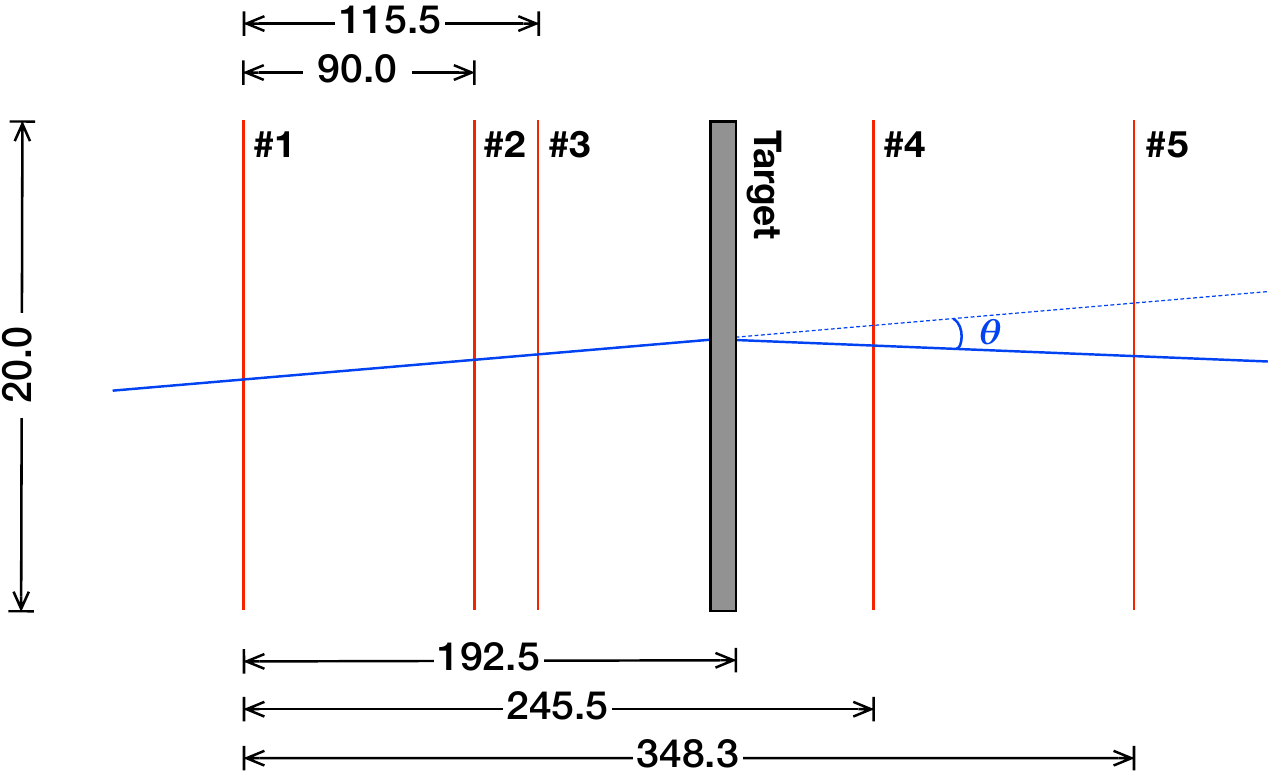
\includegraphics[width=0.6\textwidth]{Figures/muEDM_Dec2021/Positions_Telescope.png}\\
            \caption{Sketch of the telescope of Silicon Pixel Sensors used to study the multiple scattering in different materials.
            The samples are held in the position of the 'target'. 
            In this sketch, the beam is coming from the left side.}
            \label{fig:muEDM:beamtime2021:telescope}
        \end{figure}

        \begin{figure}   
            \centering
            \subfloat[Picture of the setup for the beamtime of 2021. On the right, the scintillator was used as an external trigger, on the left, beam exit window.]{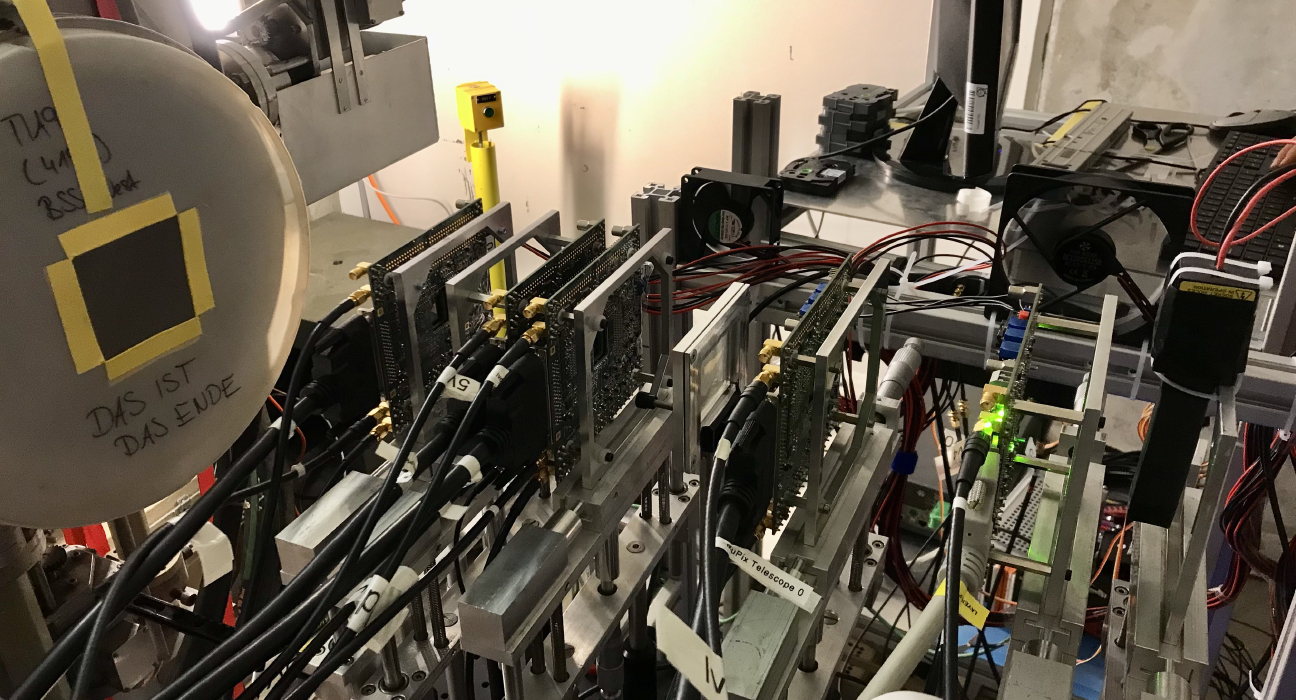
\includegraphics[height=5.5cm, keepaspectratio]{Figures/muEDM_Dec2021/Telescope_Picture.png}\label{fig:muEDM:beamtime2021:setup:telescope}}
            \hfill
            \subfloat[Picture of one of the MuPix10 mounted on the two PCBs.]{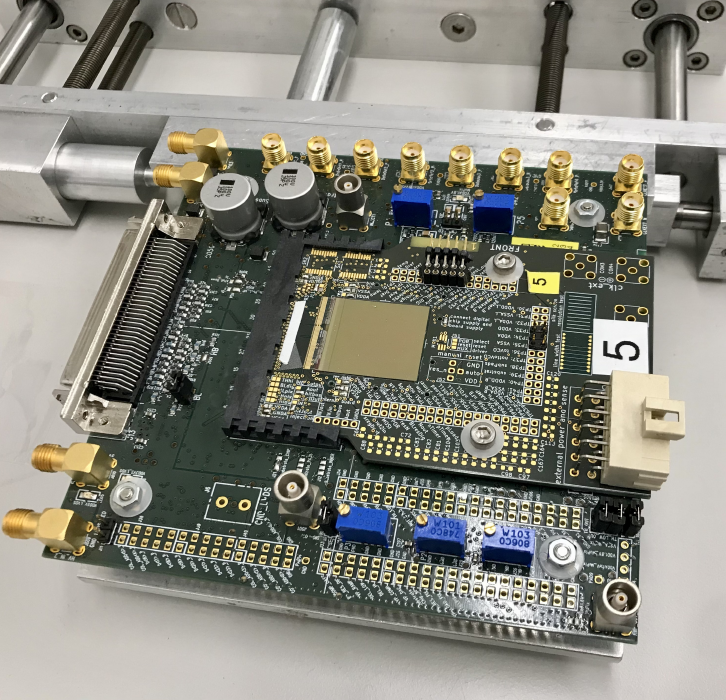
\includegraphics[height=5.5cm, keepaspectratio]{Figures/muEDM_Dec2021/MuPix10_Picture.png}\label{fig:muEDM:beamtime2021:setup:MuPix10}}
            \caption{Picture of the setup and one of the MuPix10 (grey-colored square) mounted on the PCBs.}
            \label{fig:muEDM:beamtime2021:setup}
        \end{figure}

        \begin{figure}
            \centering
            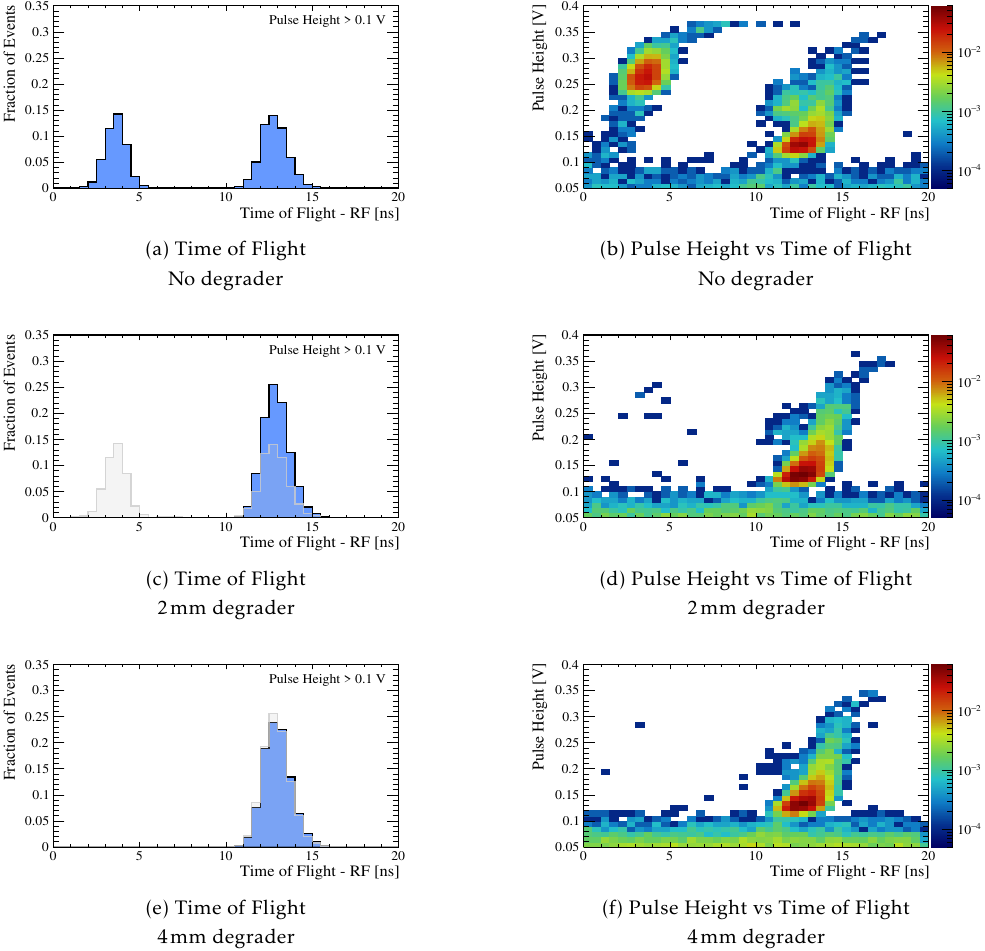
\includegraphics[width=0.9\textwidth]{Figures/muEDM_Dec2021/muEDM_beamtime2021_TOF.png}
            \caption{Timing and the 2D plot for time and pulse height for \SI{120}{MeV/c} particles. The three rows show what happens when inserting degraders of different thicknesses.
            With no degrader, the $\uppi$ peak is visible at lower TOF.
            When increasing the thickness, the contributions of $\uppi$ and $\upmu$ decrease.
            It is important to note that the $e$ and $\upmu$ distribution overlap.
            In gray the distribution of the previous plot to make a comparison.}
            \label{fig:muEDM:beamtime2021:TOF}
        \end{figure}

        \begin{table}[]
            \centering
            \begin{tabular}{c|c}
                 &  \\
                 & 
            \end{tabular}
            \caption{Table of the different materials, thicknesses, particles and momenta used.}
            \label{tab:my_label}
        \end{table}

    \status{started}
    \subsection{Data analysis}
        \paragraph{Track selection}
        Initial angular distributions obtained were broad due to noise in downstream sensors, making it difficult to distinguish noise from true hits. 
        To address this, a filtering process was developed to select the track candidate with the least spatial separation between the intersections of upstream and downstream tracks on the plane of the sample.
        The expected angular distribution for particles passing through a material at normal incidence should be spatially symmetric and independent of chosen projection axes. 
        Any deviation from this symmetry could indicate experimental, data processing, or analysis errors. 
        To mitigate the effects the idea was to combine distributions from multiple axes.
        In the initial distributions, the broad background can be attributed to false tracks generated by noise, poor fits, and some contribution of events with large angles of scattering in the telescope itself. 
        This background was suppressed by enforcing a distance of \SI{1}{mm} between the points at which the upstream and downstream tracks intersect the plane of the sample.        
        Distributions before and after applying this filter are shown in black and red in Fig.~\ref{fig:muEDM:beamtime2021:distributions}
        This distribution was then corrected for the geometric acceptance of the telescope.
        \begin{figure}
            \centering
            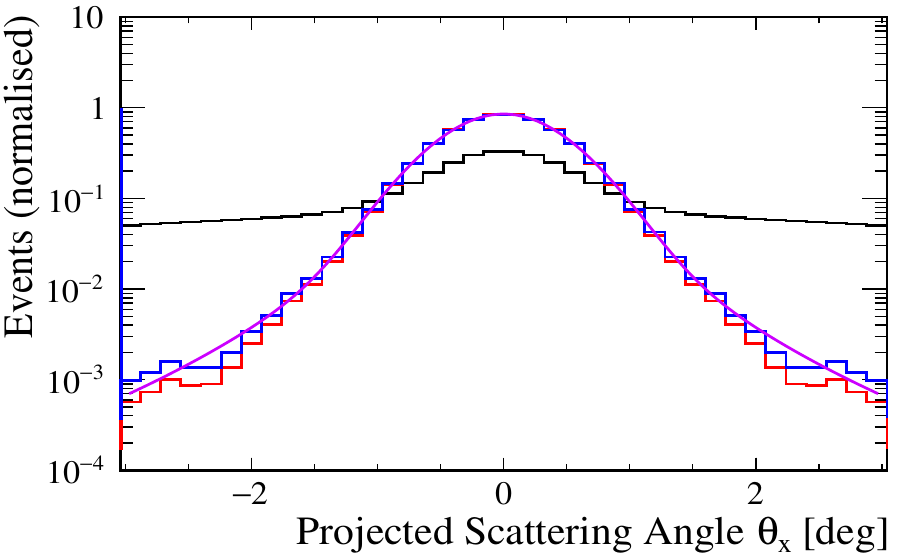
\includegraphics[width=0.8\textwidth]{Figures/muEDM_Dec2021/distributions.png}
            \caption{The angular distributions show: the full distribution (black), the distribution after cuts in the distance at the sample's plane (red), the distribution after acceptance correction (blue), and the fitted function for telescope characterization (violet).}
            \label{fig:muEDM:beamtime2021:distributions}
        \end{figure}
        
        \paragraph{Acceptance}
        The correction for the geometrical acceptance of the telescope was essential to accurately determine the tails of the angular distribution.
        To estimate the acceptance, for each upstream track identified, scattering angles were randomly assigned and added to a histogram, distinguishing instances within the acceptance of the most downstream sensor. 
        The ratio of histograms yielded the average acceptance as a function of projected scattering angles. 
        The acceptance correction was applied on a per-event basis, adjusting the scattering angles based on the acceptance value. 
        An example of such correction is shown in blue in Fig.~\ref{fig:muEDM:beamtime2021:distributions}
        
        \paragraph{Deconvolution}
        The method of track selection and acceptance correction was applied to both runs with and without the sample. 
        The distributions from these runs were then fitted.
        The process involved:
        \begin{outline}
            \1 Characterizing the telescope's response without the sample using a weighted sum of a Gaussian distribution and a Student's t distribution
            \1 Convolving the response function with the sample's angular distribution, assumed to follow a single Student's t distribution
            \1 using the negative log-likelihood to determine the best-fit parameters for describing the measured distribution with the sample
        \end{outline}
    
    \status{started}
    \subsection{Model evaluation and conclusions}
        This first beamtime aimed at testing the agreement between the Highland formula and the \gf Urb\'{a}n model for the multiple scattering in thin materials.
        The analysis of the data collected is still not finalized, but a rough agreement between data and models can be seen in Fig.~\ref{fig:muEDM:beamtime2021:results}.
        There are improvements that could be added to the analysis and/or to the simulation of the experimental setup, so updated results are expected in the following months.
        
    \begin{figure}   
            \centering
            \subfloat[Pokalon (orange), \SI{17}{\micro m} Graphite (blue), \SI{50}{\micro m} Graphite (violet), Silicon (red); circular markers for data at \SI{70}{MeV} and squared at \SI{90}{MeV}; error bars are the statistical uncertainties and the shaded area is the total uncertainties.]{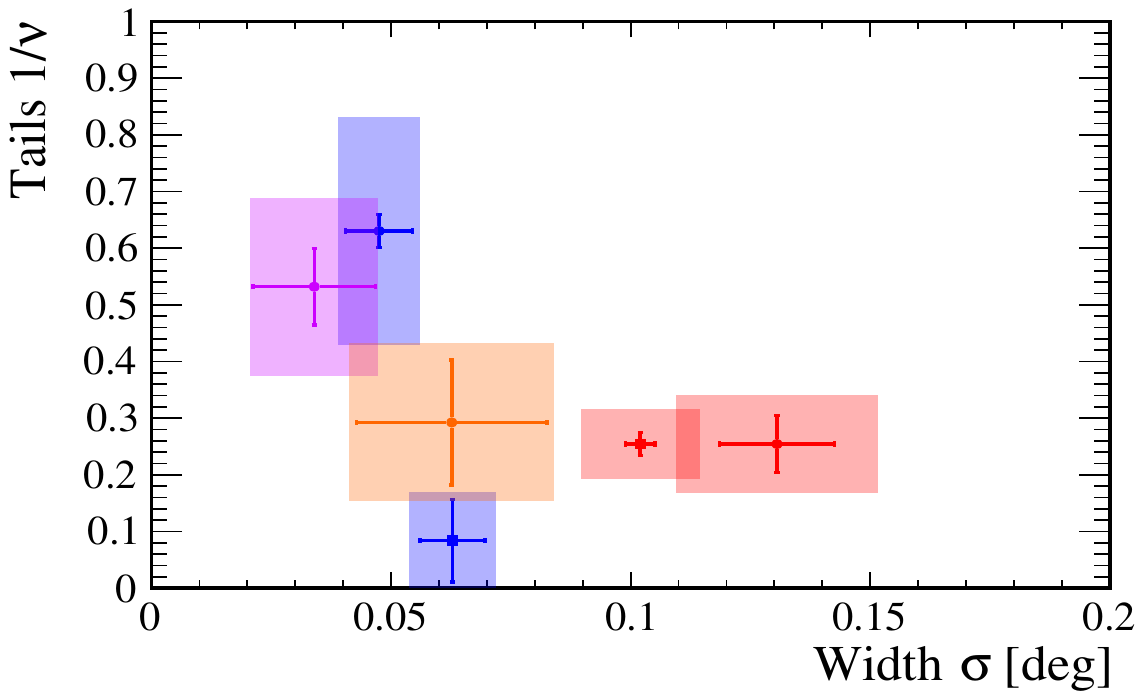
\includegraphics[width=0.48\textwidth, keepaspectratio]{Figures/muEDM_Dec2021/ms_fits.png}\label{fig:muEDM:beamtime2021:results:analysis}}
            \hfill
            \subfloat[Same color/shape coding as Fig.~\ref{fig:muEDM:beamtime2021:results:analysis} and the predictions of the Highland formula are shown by lines of width representing the uncertainty in thickness.]{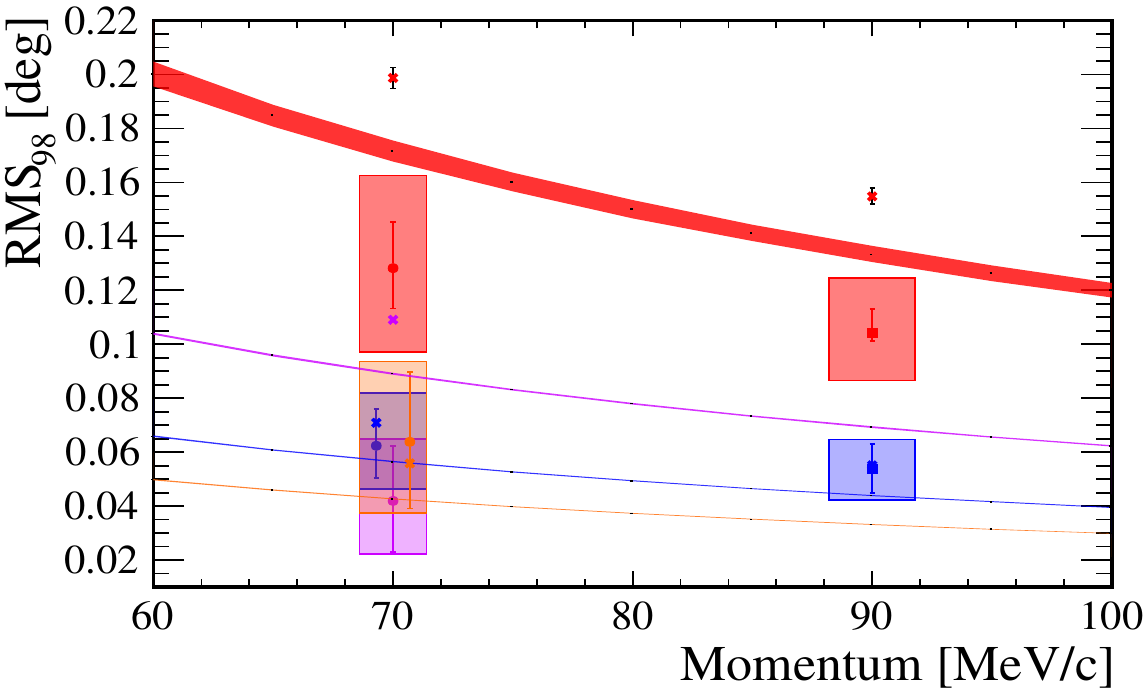
\includegraphics[width=0.48\textwidth, keepaspectratio]{Figures/muEDM_Dec2021/gf-highland_evaluation.png}\label{fig:muEDM:beamtime2021:results:models}}
            \caption{Results of the analysis of the different samples and confronted with predictions using the Highland formula and \gf. The details are not easy to read but the 'bring-home' message is that the results are somewhat in agreement and some improvement are planned on the analysis.}
            \label{fig:muEDM:beamtime2021:results}
        \end{figure}
        
\section{Beamtime 2022: Telescope and entrance detector}
    \subsection{Construction}
    \begin{figure}   
            \centering
            \subfloat[Custom feed-throughs: PCB board, with soldered connectors, sealed with Stycast in a blind flange.]{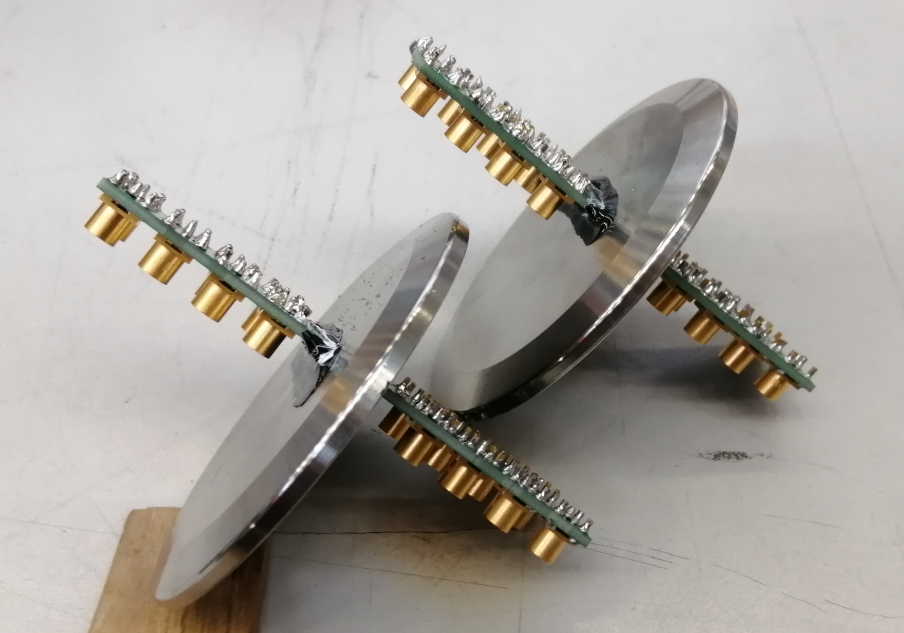
\includegraphics[width=0.49\textwidth, keepaspectratio]{Figures/muEDM_Nov2022/feedthrough.png}\label{}}
            \hfill
            \subfloat[A small PCB board with 3 SiPMs and one connector attached with optical cement to one of the scintillators.]{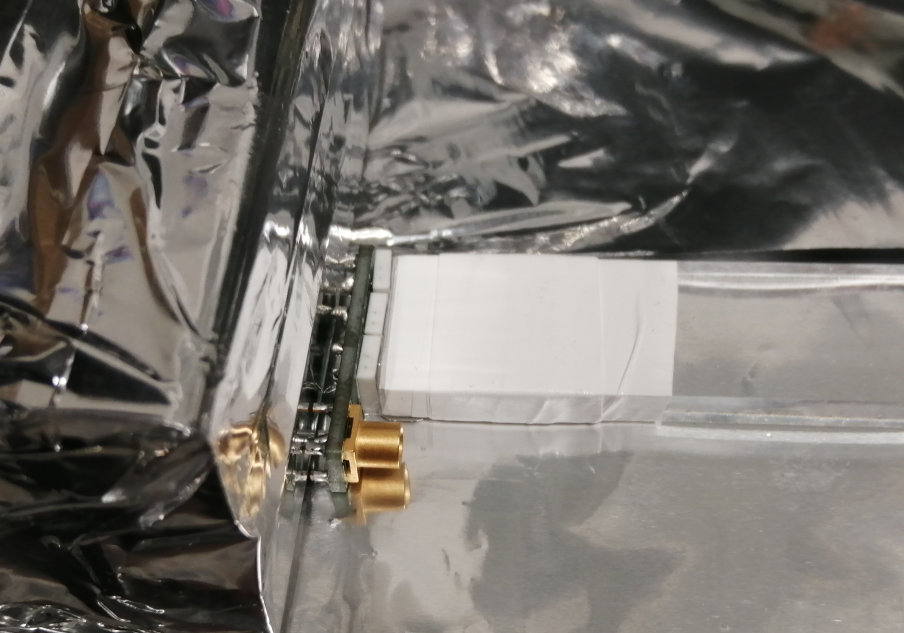
\includegraphics[width=0.49\textwidth, keepaspectratio]{Figures/muEDM_Nov2022/SIPMgluing.png}\label{}}
            \caption{asd}
            \label{fig:muEDM:beamtime2021:setup}
        \end{figure}
        
        \begin{figure}   
            \centering
            \subfloat[]{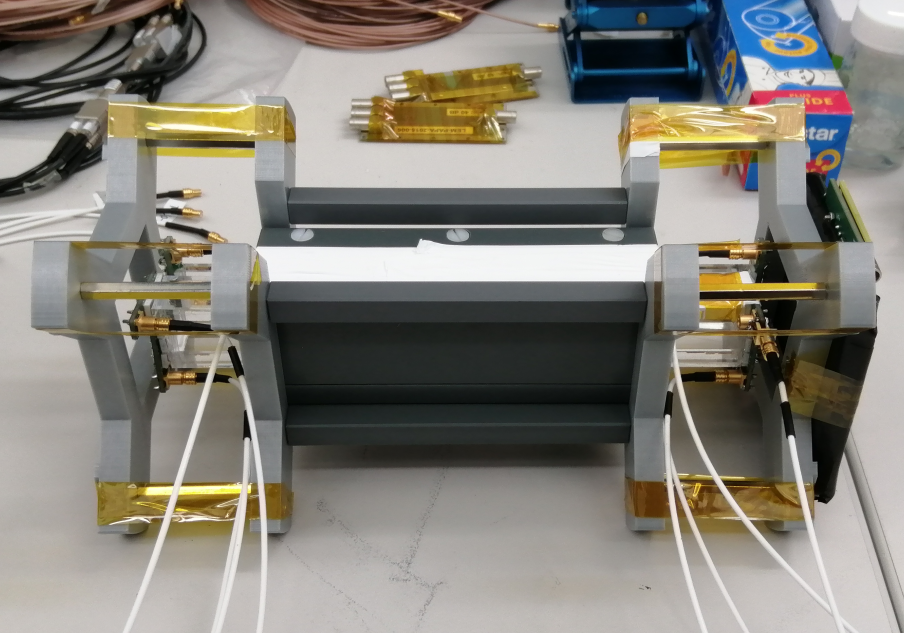
\includegraphics[width=0.49\textwidth, keepaspectratio]{Figures/muEDM_Nov2022/telescope_side.png}\label{}}
            \hfill
            \subfloat[]{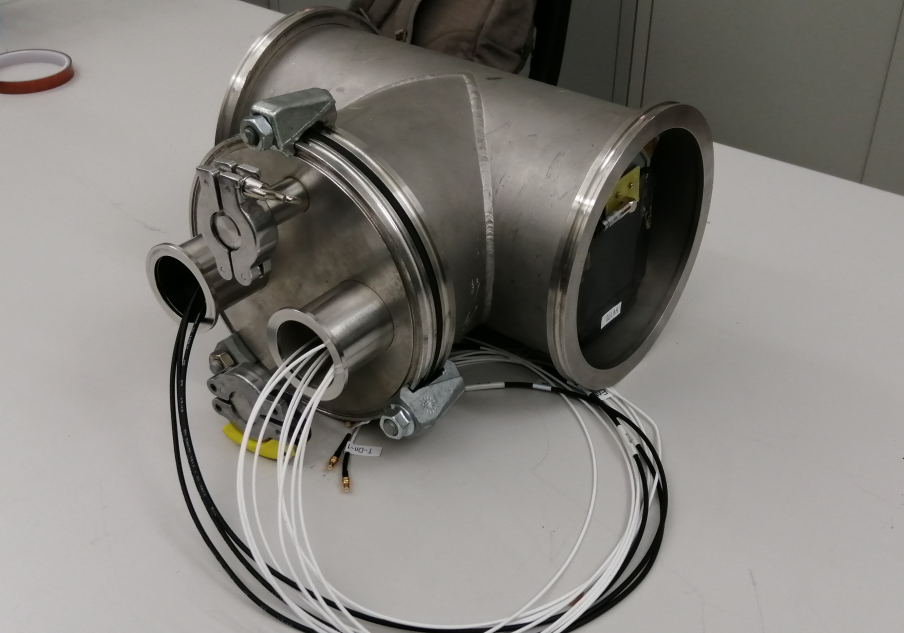
\includegraphics[width=0.49\textwidth, keepaspectratio]{Figures/muEDM_Nov2022/telescope_built.png}\label{}}
            \caption{asd}
            \label{fig:muEDM:beamtime2021:setup}
        \end{figure}
    \subsection{Data taking}
    \subsection{Data analysis}
\section{Beamtime 2023: Multi readout entrance}
    \subsection{Data taking}
    \subsection{Data analysis}

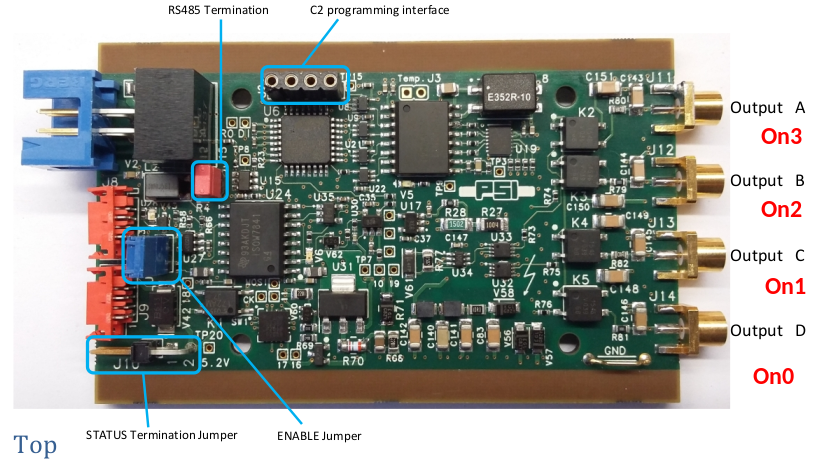
\includegraphics[width=0.8\textwidth]{Figures/muEDM_Dec2021/HV.png}\\
\subsection{Describe the beam}
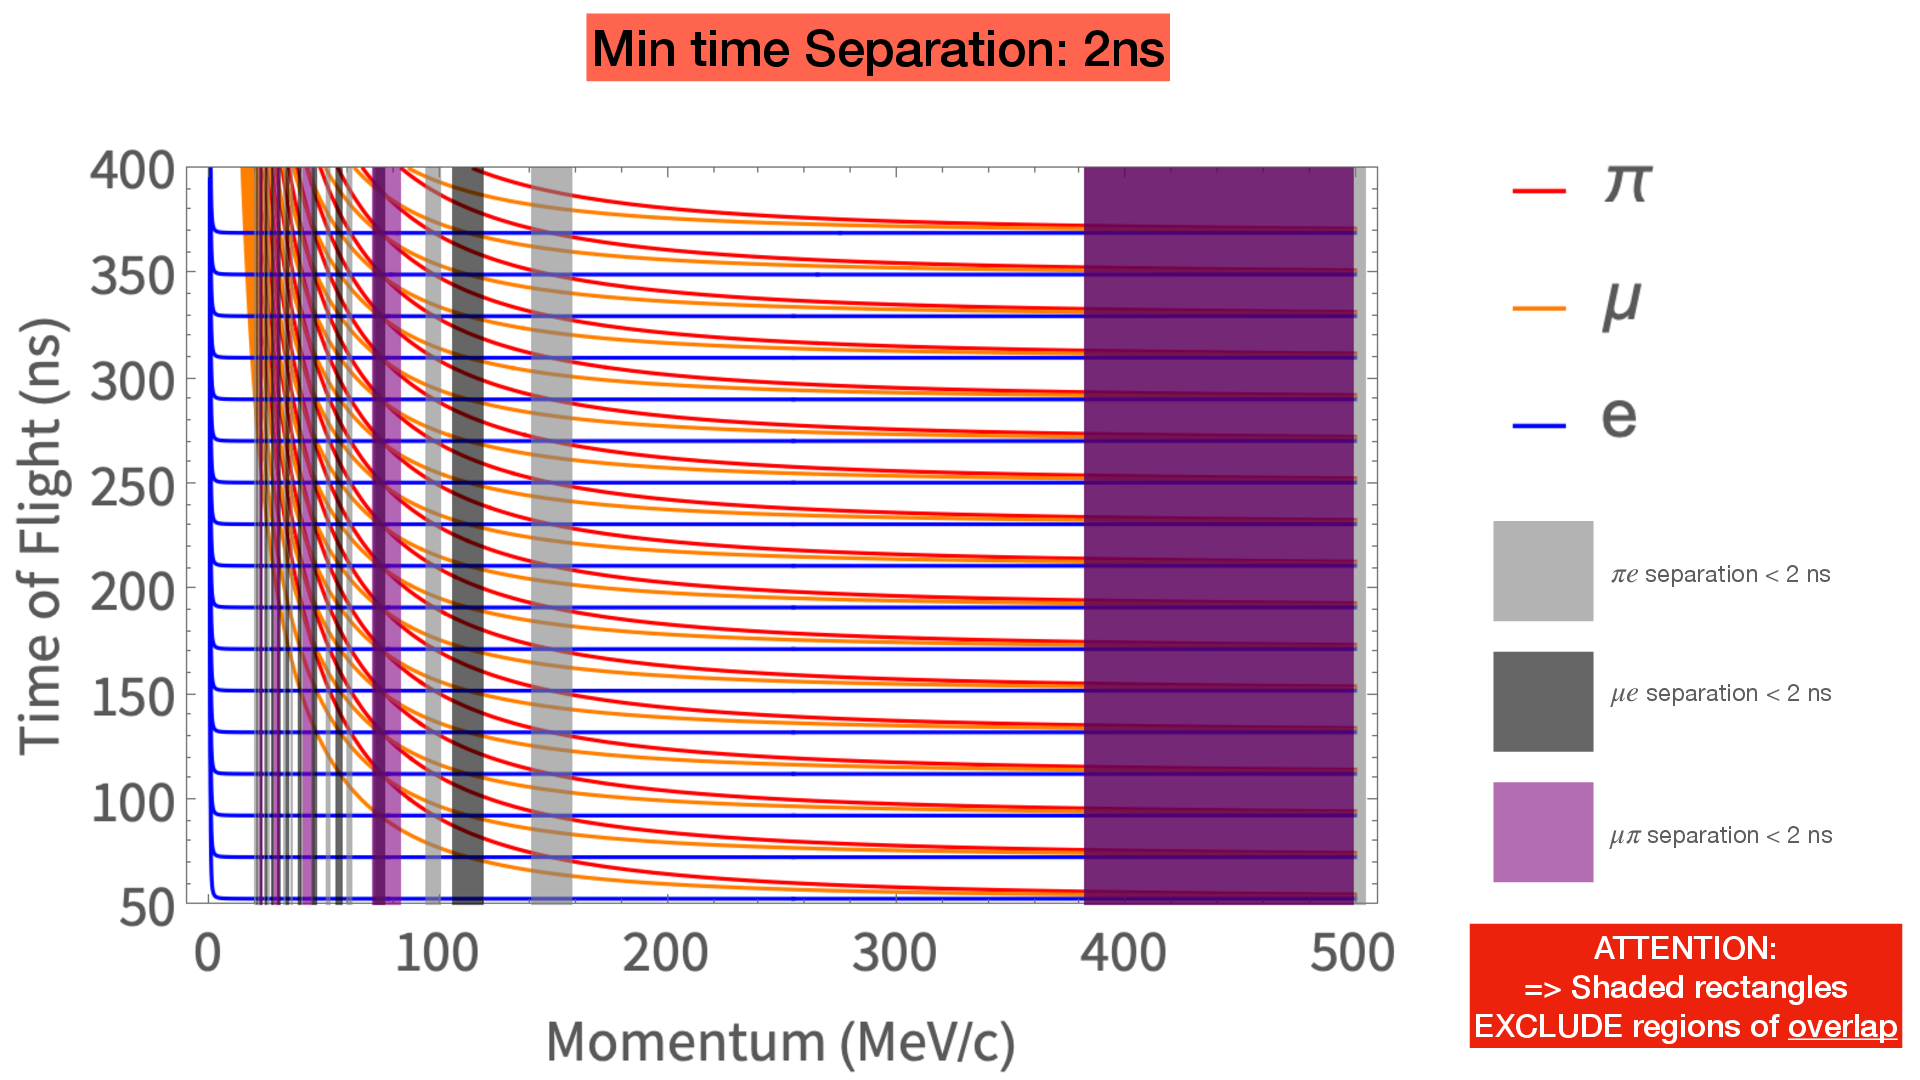
\includegraphics[width=0.8\textwidth]{Figures/muEDM_Dec2021/ToFPlots-0.png}\\

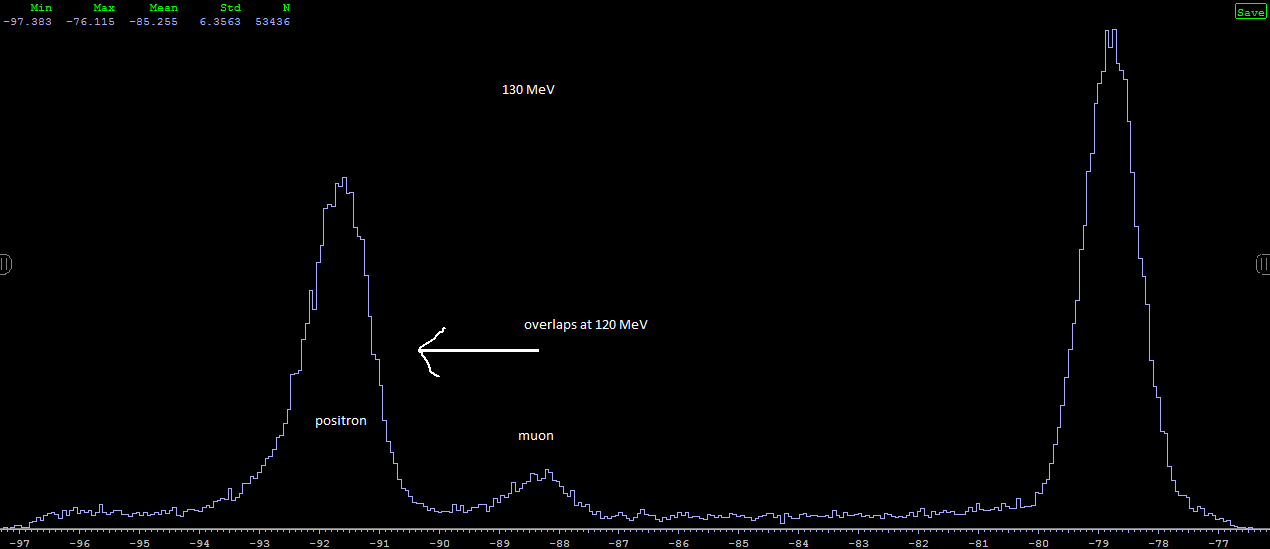
\includegraphics[width=0.8\textwidth]{Figures/muEDM_Dec2021/TOFAllEnergies130.png}\\
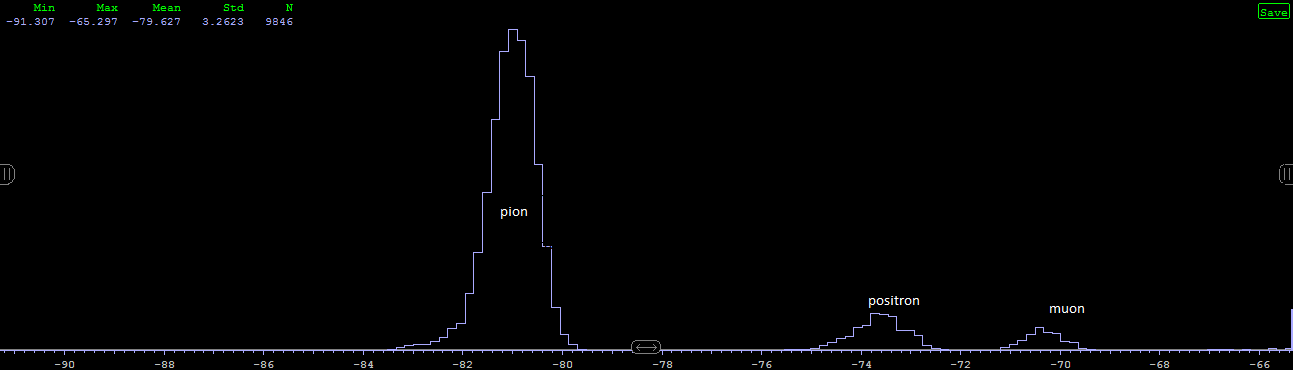
\includegraphics[width=0.8\textwidth]{Figures/muEDM_Dec2021/TOFMediumCut125.png}
\section{Conclusions}

\status{started}
\printbibliography[
    heading = bibliographychapter,
    title=Bibliography on muEDM entrance detector
]

\end{refsection}


